\documentclass[../report.tex]{subfiles}

\begin{document}

\graphicspath{{img/}{../img/}}

\section{Scrum men... Ikke helt}
\label{sec:Scrum}

Target-projektgruppen har valgt at arbejde med Scrum i deres implementeringsfase hvilket optager cirka halvdelen af deres tidsplan(se Gantt diagram fig \ref{fig:Gantt} side \pageref{fig:Gantt}).


\paragraph{Hvad er Scrum?}
Scrum er en agil softwareudviklingsmetode, hvis hovedm�l er h�ndteringen af l�bende �ndringer i kravspecifikationen. Indenfor h�ndtering af �ndringer er Scrums mods�tning vandfaldsmodellen, som ikke tager sig p�nt i et milj� med mange krav�ndringer.

\paragraph{Scrum men... Hvad mangler s�?}
I target-projektet bliver der arbejdet efter Scrum, men ikke Scrum i dets fulde forstand. Det blev besluttet at k�re l�st p� nogle af Scrums discipliner, fordi der var enighed om at det ikke gav meget mening for en projektgruppe der kun m�des et par gange om ugen. Se figur \ref{fig:Scrum} p� side \pageref{fig:Scrum} for en oversigt over aktiviteter og figur \ref{fig:ScrumTimeline} p� side \pageref{fig:ScrumTimeline} for en tidslinje. \\

\begin{figure}[H]
\centering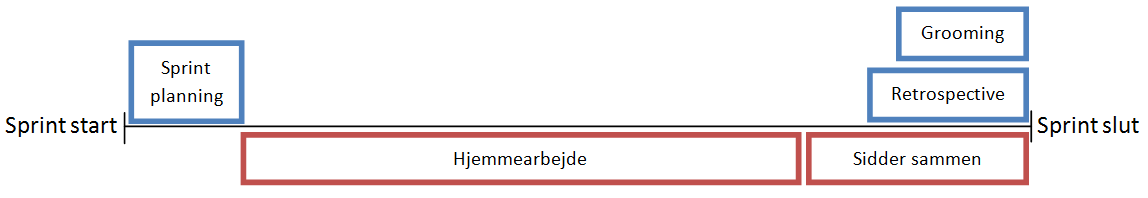
\includegraphics[scale=0.45]{SCRUMtimeLine.png}
\caption{Sprint tidslinje}
\label{fig:ScrumTimeline}
\end{figure}

\begin{figure}[H]
\begin{tabularx}{14cm}{c|X}
\textbf{Aktivitet}  & \textbf{Beskrivelse} \\
Scrum roller & I et eksamensprojekt er det urealistisk at have en person til kun at v�re product owner. I target-projektet er product owner ene og alene ansvarlig for kommunikation med stakeholders og prioritering af product items, men han er ogs� udvikler i Scrum teamet. Derudover er Scrummaster og developers blevet brugt klassisk.     \\ 
 & \\
Standup meeting & Der blev ikke afholdt nogen standup meetings. \\
 & \\
Grooming & Den n�stsidste aktivitet var grooming, hvor Scrumboardet blev ryddet op. \\
 & \\
Retrospective & Den sidste aktivitet var retrospective. Gruppen benyttede Keep-Stop-New metoden\footnote{http://www.mountaingoatsoftware.com/agile/scrum/sprint-retrospective/}. \\
 & \\
Sprint planning & Den f�rste aktivitet i hvert sprint er en klassisk sprint planning. Tasks blev estimeret med planning poker i points som beskrevet i afsnit \ref{sec:PERT} p� side \pageref{sec:PERT}. \\
 & \\
Scrumboard & Scrum boardet er den centrale oversigt over aktiviteter. Da target-projektgruppen ikke havde et fast lokale allokeret, var et fysisk Scrumboard ikke muligt, s� online v�rkt�jet Trello\footnote{Trello.com} blev brugt i stedet. \\
 & \\
Tidtagning & Der blev i fire sprints taget tid p� arbejdet med Toggl\footnote{Toggl.com}. Target-projektgruppen blev bedt om dette for hj�lp med analyse i dette projekt.\\
 & \\
\end{tabularx}
\caption{Target-projektets aktiviteter}
\label{fig:Scrum}
\end{figure} 

Target-projektgruppen har ikke brugt Scrum i hele deres projektforl�b, men det kunne de godt have valgt at g�re. Inden Scrumforl�bet ser vi fra Gantt diagrammet p� fig \ref{fig:Gantt} at gruppen har arbejdet med Businesscase og Requirements.

\begin{quote}
\textit{"Grunden til at vi ikke har brugt Scrum fra projektstart er, at vi f�lte en hvis struktur af dokumentationen var n�devendig. Vi har alts� set p� Scrum som en implementerings procesmodel. I vores Scrum forl�b har vi dog ogs� haft andet end implementeringstasks, og vi ser sagtens gevinster ved at bruge Scrum fra projektstart."}
\end{quote}

\end{document}